\documentclass[a4paper,UKenglish,cleveref, autoref]{lipics-v2019}
\usepackage{proof}
\usepackage{tikz}
\usepackage{gensymb}


\usetikzlibrary{automata,trees,calc,arrows.meta,positioning,decorations.pathreplacing,bending,shapes.geometric, intersections, hobby}
%This is a template for producing LIPIcs articles. 
%See lipics-manual.pdf for further information.
%for A4 paper format use option "a4paper", for US-letter use option "letterpaper"
%for british hyphenation rules use option "UKenglish", for american hyphenation rules use option "USenglish"
%for section-numbered lemmas etc., use "numberwithinsect"
%for enabling cleveref support, use "cleveref"
%for enabling cleveref support, use "autoref"


%\graphicspath{{./graphics/}}%helpful if your graphic files are in another directory

\bibliographystyle{plainurl}% the mandatory bibstyle

\title{Towards a Formalisation of Cook's Theorem} %TODO Please add

\titlerunning{}%optional, please use if title is longer than one line

\author{Lennard Gäher}{Saarland University, Germany}{s8legaeh@stud.uni-saarland.de}{}{}%TODO mandatory, please use full name; only 1 author per \author macro; first two parameters are mandatory, other parameters can be empty. Please provide at least the name of the affiliation and the country. The full address is optional

\authorrunning{L. Gäher}%TODO mandatory. First: Use abbreviated first/middle names. Second (only in severe cases): Use first author plus 'et al.'

\Copyright{Lennard Gäher}%TODO mandatory, please use full first names. LIPIcs license is "CC-BY";  http://creativecommons.org/licenses/by/3.0/

%\ccsdesc[100]{General and reference~General literature}
%\ccsdesc[100]{General and reference}%TODO mandatory: Please choose ACM 2012 classifications from https://dl.acm.org/ccs/ccs_flat.cfm 

%\keywords{Dummy keyword}%TODO mandatory; please add comma-separated list of keywords

%\category{}%optional, e.g. invited paper

\relatedversion{}%optional, e.g. full version hosted on arXiv, HAL, or other respository/website
%\relatedversion{A full version of the paper is available at \url{...}.}

\supplement{}%optional, e.g. related research data, source code, ... hosted on a repository like zenodo, figshare, GitHub, ...

%\funding{(Optional) general funding statement \dots}%optional, to capture a funding statement, which applies to all authors. Please enter author specific funding statements as fifth argument of the \author macro.


\nolinenumbers %uncomment to disable line numbering

\hideLIPIcs  %uncomment to remove references to LIPIcs series (logo, DOI, ...), e.g. when preparing a pre-final version to be uploaded to arXiv or another public repository

%Editor-only macros:: begin (do not touch as author)%%%%%%%%%%%%%%%%%%%%%%%%%%%%%%%%%%
\EventEditors{John Q. Open and Joan R. Access}
\EventNoEds{2}
\EventLongTitle{42nd Conference on Very Important Topics (CVIT 2016)}
\EventShortTitle{CVIT 2016}
\EventAcronym{CVIT}
\EventYear{2016}
\EventDate{December 24--27, 2016}
\EventLocation{Little Whinging, United Kingdom}
\EventLogo{}
\SeriesVolume{42}
\ArticleNo{23}
%%%%%%%%%%%%%%%%%%%%%%%%%%%%%%%%%%%%%%%%%%%%%%%%%%%%%%

\usepackage{gensymb}
\newcommand*{\listsofb}[1]{\mathcal{L} (#1)}
\newcommand*{\listsof}{\mathcal{L}~}

\newcommand{\None}{\emptyset}
\newcommand{\Some}[1]{\degree\kern-0.5ex#1}

\newcommand*{\match}{\textbf{match}~}
\newcommand*{\withl}{\textbf{[}~}
\newcommand*{\withr}{~\textbf{]}}
\newcommand*{\withm}{\quad\textbf{|}\quad}
\newcommand*{\llet}{\textbf{let}~}
\newcommand*{\lin}{\textbf{in}~}
\newcommand{\ITE}[3]{\textbf{if}~{#1}~\textbf{then}~{#2}~\textbf{else}~{#3}}

\newcommand{\Type}{\textsf{\bfseries T}}
\newcommand{\Prop}{\textsf{\bfseries P}}
\newcommand{\bool}{\textsf{B}}
\newcommand{\btrue}{\mathsf{T}}
\newcommand{\bfalse}{\mathsf{F}}
\newcommand{\andb}{\&\&}
\newcommand{\orb}{||}
\newcommand{\notb}{!}
\newcommand{\nat}{\mathsf{N}}
\newcommand{\natS}{1 + }
\newcommand{\length}[1]{|#1|}

\newcommand{\con}{\mathop{{+}\!\!\!{+}}}
\newcommand{\rev}{\mathsf{rev}}
\newcommand{\opt}[1]{\mathcal{O}{#1}}
\newcommand{\nil}{[]}

\newcommand{\eqb}[2]{#1\overset{?}{=}#2}

\newcommand{\bnfmid}{~\mid~}

\newcommand{\concat}{\con}


\newcommand{\TODO}[1]{}

\newcommand{\strent}{\rightsquigarrow}
\newcommand{\constrent}{\overset{!}{\rightsquigarrow}}
\newcommand{\Rfinal}{R_{\text{final}}}

\begin{document}

\maketitle

%TODO mandatory: add short abstract of the document
\begin{abstract}
  We present an outline of the planned proof of Cook's Theorem in Coq.
\end{abstract}

\newcommand{\gennp}{\textbf{GenNP}}
\newcommand{\strconrew}[1]{$\textbf{StrConRew}_{#1}$}
\newcommand{\csat}{\textbf{CSAT}}
\newcommand{\sat}{\textbf{SAT}}
\newcommand{\NP}{\textsf{NP}}

\section{Introduction}
Cook's Theorem was proved in 1971 by Stephen A.\ Cook (and, in parallel, by Levin) and is one of the foundational results of computational complexity theory. 
It states that the satisfiability problem on CNFs \textbf{SAT} is NP-hard, that is, any problem $Q \in NP$ can be polynomial-time reduced to it: $Q \prec_{\text{p}} \textbf{SAT}$. 
There are multiple well-known textbook proofs available. We strive to adapt a particularly simple one which encodes the transitions of a Turing machine using logical formulas layed out in a tableau.
An outline of this classical proof can be found in~\cite{Sipser:TheoryofComputation}. 

Our reduction has the following structure: 
\begin{center}
  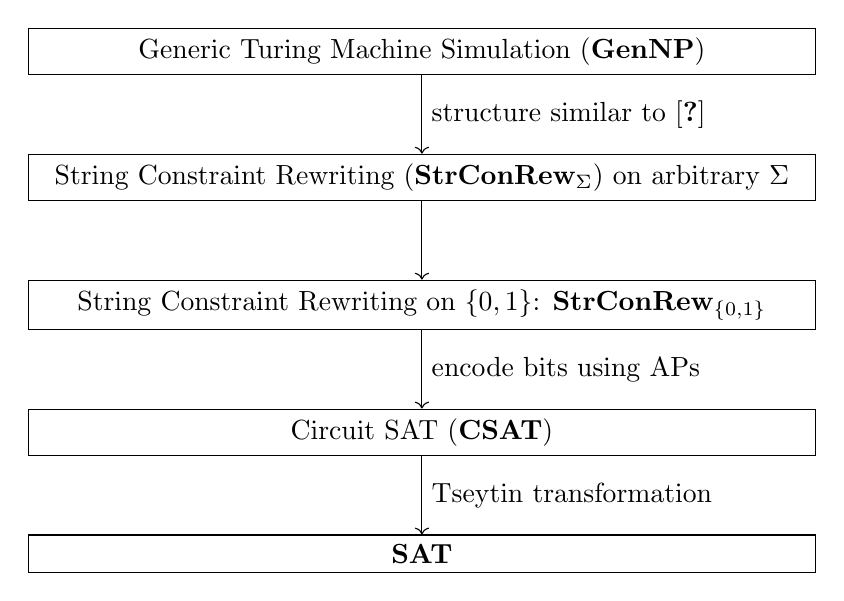
\begin{tikzpicture}
    \node[rectangle, draw=black, minimum width = 10cm] (gennp) {Generic Turing Machine Simulation (\textbf{GenNP})};
    \node[rectangle, draw=black, below = of gennp, minimum width = 10cm] (strrew1) {String Constraint Rewriting ($\textbf{StrConRew}_\Sigma$) on arbitrary $\Sigma$};
    \node[rectangle, draw=black, below = of strrew1, minimum width = 10cm] (strrew2) {String Constraint Rewriting on $\{0, 1\}$: $\textbf{StrConRew}_{\{0,1\}}$};
    \node[rectangle, draw=black, below = of strrew2, minimum width = 10cm] (csat) {Circuit SAT (\textbf{CSAT})};
    \node[rectangle, draw=black, below = of csat, minimum width = 10cm] (sat) {\textbf{SAT}};
    \draw[->] 
      (gennp) edge node[right] {structure similar to~\cite{Sipser:TheoryofComputation}} (strrew1)
      (strrew1) edge (strrew2)
      (strrew2) edge node[right] {encode bits using APs} (csat)
      (csat) edge node[right] {Tseytin transformation} (sat);
  \end{tikzpicture}
\end{center}

The reduction from \gennp{} to \strconrew{\Sigma} does the main job of encoding the behaviour of Turing machines. We are then left with a structurally much simpler problem on strings. 
In order to be able to encode this problem using logical formulas, we then simplify the alphabet to $\{0, 1\}$ in a reduction to \strconrew{\{0, 1\}}, making it possible to encode single characters using a boolean-valued atomic proposition in the reduction to \csat. The encoding of the string rewriting system that we use will not be in conjunctive normal form (CNF), therefore we then use the Tseytin transformation in a reduction from \csat{} to \sat{} on CNFs. 

\section{Reduction of \textbf{GenNP} to $\textbf{StrConRew}_\Sigma$}
We first give a formal description of the two involved problems. 

\subsection*{Generic Turing Machine Simulation (\gennp)}
\begin{definition}
  Given a deterministic 1-tape Turing machine $M$ and numbers $k$ and $t$, decide whether there is an input $x$ of length $\length{x} \le k$ such that $M$ halts on $x$ in at most $t$ steps.
\end{definition}

A more wide-spread (but equivalent) definition of a generic problem for Turing machines is the following: Given a nondeterministic Turing machine $M$ and an input $x$ and a number $t$, decide whether $M$ halts on $x$ in at most $t$ steps. 
We do not use this variant since it would require us to formalise the notion of nondeterminism. Instead, our definition builds on the well-known verifier characterisation of \NP{}. The whole input of the Turing machine is regarded as a certificate; the instance itself can be statically encoded in the states of the Turing machine.

The restriction to 1-tape Turing machines is without loss of generality, a fact which has also been formalised in Coq~\cite{TODO}. 

Using a classical definition of the complexity class \NP{} using Turing machines, one is easily convinced that \gennp{} is \NP{}-hard. For our definition using the call-by-value $\lambda$-calculus L, this isn't straightforward at all, though. We thus leave the problem of proving the \NP{}-hardness of \gennp{} open for now.

\subsection*{String Constraint Rewriting (\strconrew{\Sigma})}
This problem works on strings of a fixed length $l$ over an alphabet $\Sigma$. Starting with an initial string $x_0$, the task is to determine whether there is a sequence of strings $x_1, \ldots, x_t$ such that $x_{i+1}$ validly follows from $x_i$, denoted by $x_i \strent x_{i+1}$, such that $x_t$ satisfies a final condition. The relation $x_i \strent x_{i+1}$ is described by a set $R$ of rewrite windows.

Each window specifies a rewrite constraint $a \constrent b$ for strings $a, b$ of a fixed length $w \le l$: If the string $a$ matches a substring of $x_i$, then in the string $x_{i+1}$ this substring must be replaced by $b$. 
Formulated differently, in order for a string $x_{i+1}$ to validly follow from a string $x_i$, each rewrite window $a \constrent b$ must hold at every possible offset in $x_i$:
\[\bigwedge_{(a \constrent b) \in R} \bigwedge_{0 \le j \le l - w + 1} (x_i[j..j+w-1] = a \rightarrow x_{i+1}[j..j+w-1] = b) \]

The final condition is given by a set of substring constraints $\Rfinal$: In order for the final string $x_t$ to be valid, there needs to be $x \in \Rfinal$ such that $x$ is a substring of $x_t$:
\[\bigvee_{x \in \Rfinal} \bigvee_{0 \le j \le l - \length{x} + 1} (x_t[j..j+\length{x} -1] = x) \]

\newcommand*{\validR}{\textsf{valid}}

We now formally define \strconrew{\Sigma}:
\begin{definition}
  Given: 
  \begin{itemize}
    \item a width $w$ of rewrite windows, 
    \item a string length $l$,
    \item a step count $t$,
    \item an initial string $x_0 \in \Sigma^l$,
    \item a list of rewrite windows $R = \{a_i \constrent b_i | i \in \nat \land a_i, b_i \in \Sigma^w\}$,
    \item a set of final substring constraints $\Rfinal = \{f_i | i \in \nat \land \exists k \le l, f_i \in \Sigma^k\}$
  \end{itemize}

  Determine if there is a sequence of strings $x_1, \ldots, x_t \in \Sigma^l$ such that 
  \begin{itemize}
    \item For every $0 \le i < t$ it holds that $\validR(x_i, x_{i+1})$, where $\validR$ is defined as follows:
      \[\forall (a \constrent b) \in R, \forall (0 \le j \le l -k + 1), x_i[j..j+ k-1] = a \rightarrow x_{i+1}[j..j+k-1] = b \]
    \item There exists an $x \in \Rfinal$ such that $x$ is a substring of $x_t$, i.e. there is $0 \le j \le l - \length{x} + 1$ with $x = x_t[j..j+\length{x} - 1]$ .
  \end{itemize}
\end{definition}

\subsection*{Reducing \gennp{} to \strconrew{\Sigma}}

\bibliography{memo}{}


\end{document}
